\documentclass[a4paper, 12pt]{article}
\usepackage{geometry}
\geometry{verbose,a4paper,tmargin=2cm,bmargin=2cm,lmargin=2cm,rmargin=2cm}
\usepackage{fontspec}
\setmainfont[
  Ligatures=TeX,
  Extension=.otf,
  UprightFont=*-regular,
  ItalicFont=*-italic,
  BoldFont=*-bold,
  BoldItalicFont=*-bolditalic,
]{xits}
\usepackage[english,russian]{babel}

\newif\ifisinsp
\newif\ifisone
\newif\ifisname
\newif\ifisnum
\isinsptrue
\isonetrue
\isnamefalse
\isnumtrue

\def \labtype {Лабораторная}
% Это для нумерации страниц после титульника
\usepackage{fancyhdr}
\pagestyle{fancy}
\renewcommand{\headrulewidth}{0pt}
\fancyfoot[C] {\thepage}

\usepackage{hyperref}
\hypersetup{pdftex,colorlinks=true,allcolors=black}
\usepackage{hypcap}

\usepackage{graphicx}
\usepackage{adjustbox}
\usepackage{multirow}

\def \labtype {Курсовая}
\def \labsubj {Системы баз данных}
\def \labauthor {Айтуганов Д. А. \\ Чебыкин И. Б.}
\def \labgroup {P3301}
\def \labinsp {Беликов П. А.}
\def \labname{Разработка базы данных интернет-магазина}
\isonefalse
\isnametrue
\isnumfalse

\usepackage[dvipsnames]{xcolor}
\usepackage{fancyvrb}
\usepackage{graphicx}
\usepackage{xunicode}
\usepackage{xltxtra}
\setmonofont{DejaVu Sans Mono}
\RecustomVerbatimCommand{\VerbatimInput}{VerbatimInput} { fontsize=\scriptsize,
 %
 frame=lines,  % top and bottom rule only
 framesep=2em, % separation between frame and text
 rulecolor=\color{Gray},
 %
 label=\fbox{\color{Black}source},
 labelposition=topline,
 %
}

\begin{document}
\begin{titlepage}
	\begin{center}
		\large
		Университет ИТМО

		\vspace{0.25cm}
		
		Факультет программной инженерии и компьютерной техники
		
		Кафедра вычислительной техники
		\vfill
		
		\textsc{\labtype\spaceработа \ifisnum № \labnum{} \fi по дисциплине \\"\labsubj" \ifisname\small \\ \labname \fi}
			
		\bigskip
	\end{center}
	\vfill
	\vfill
	
	\begin{flushright}
	\ifisone
	Выполнил: \labauthor
	\else
	Выполнили: \labauthor
	\fi

	\vspace{0.25cm}
	Группа: \labgroup
			
	\vspace{0.25cm}
	\ifisinsp
	Проверяющий: \labinsp
	\fi
	\end{flushright}
	\vfill
	
	\begin{center}
	СПб, \the\year
	\end{center}
\end{titlepage}

\tableofcontents
\newpage
\section{Описание предметной области}
В качестве предметной области был выбран интернет-магазино, который продает
различные товары и имеет точки выдачи товаров.
В модели учитываются расписание сотрудников, логирование
продаж, категории товаров и т. д.

\section{Модели реализованных баз данных или репрезентативные примеры данных}

\subsection{Общая схема}
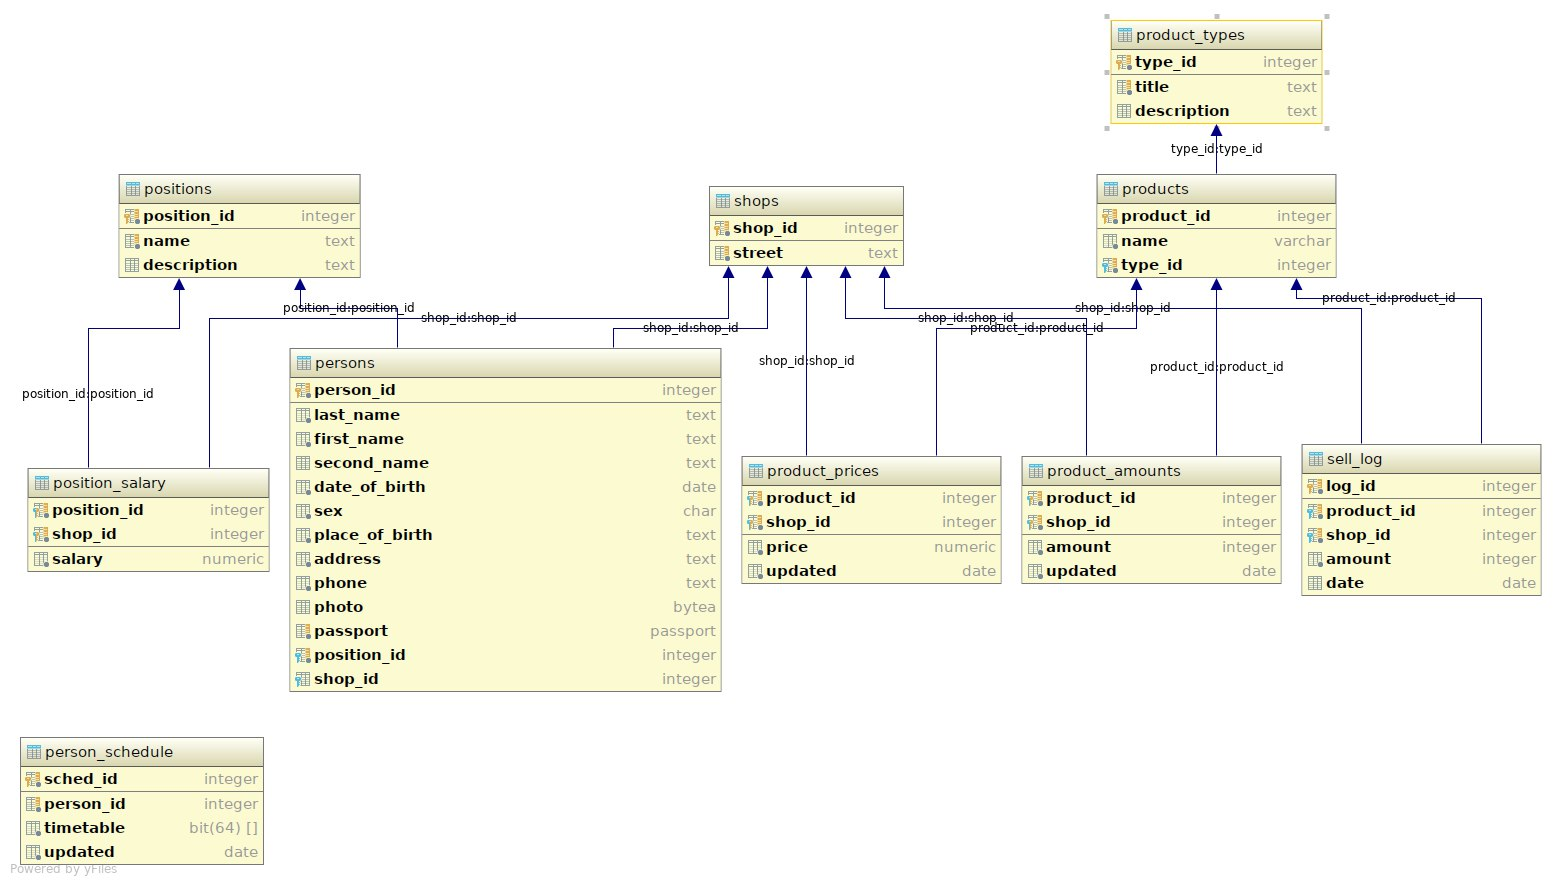
\includegraphics[width=500bp]{img/diagram.jpg}

\subsection{Представление в графовой базе данных}
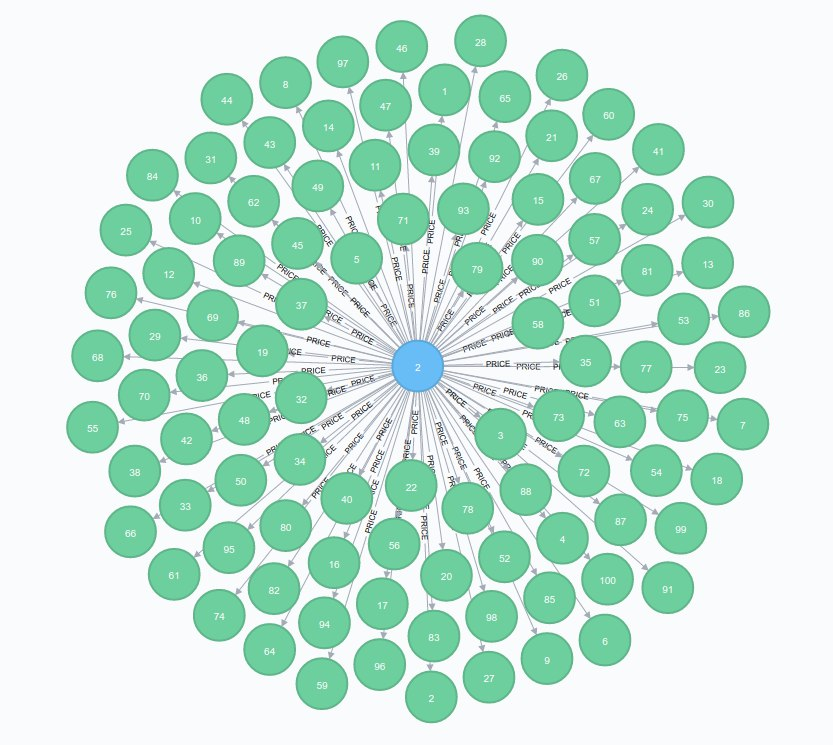
\includegraphics[width=400bp]{img/graph.jpg}


\section{Описание программных модулей в формате комментариев к коду}

ConfigurationModule -- подгружает данные конфигураций БД из файлов
\begin{Verbatim}[fontsize=\scriptsize]
package coursework.configuration;

import com.google.inject.AbstractModule;

public class ConfigurationModule extends AbstractModule {

    @Override
    protected void configure() {
        bind(AppConfiguration.class);
    }
}


// Класс, описывающий конфигурацию
@Singleton
public class AppConfiguration {

    public static final String DEFAULT_CONFIG_FILE = "default.properties";

    // Database
    public static final String DATABASE_DATASOURCE_NAME = "database.dataSourceName";
    public static final String DATABASE_SERVER_NAME     = "database.serverName";
    public static final String DATABASE_SPBSERVER_NAME  = "database.SPbServerName";
    public static final String DATABASE_DATABASE_NAME   = "database.databaseName";
    public static final String DATABASE_FIRST_NODE_IP   = "database.firstNodeIp";
    public static final String DATABASE_SECOND_NODE_IP  = "database.secondNodeIp";
    public static final String DATABASE_THIRD_NODE_IP   = "database.thirdNodeIp";
    public static final String DATABASE_BALANCER_IP   = "database.balancerIp";

    public static final String DATABASE_USER            = "database.user";
    public static final String DATABASE_PASSWORD        = "database.password";
    public static final String DATABASE_MAX_CONNECTIONS = "database.maxConnections";

    public static final String DATABASE_POSTGRESQL_PORT = "database.postgresqlPort";
    public static final String DATABASE_MONGODB_PORT    = "database.mongodbPort";
    public static final String DATABASE_NEO4J_PORT      = "database.neo4jPort";
    public static final String DATABASE_CASSANDRA_PORT  = "database.cassandraPort";
    public static final String DATABASE_CASSANDRA_SECOND_NODE_PORT  = "database.cassandraSecondNodePort";
    public static final String DATABASE_CASSANDRA_THIRD_NODE_PORT  = "database.cassandraThirdNodePort";
    public static final String DATABASE_REDIS_PORT      = "database.redisPort";

    private final Logger log = LoggerFactory.getLogger(AppConfiguration.class);

    private final ImmutableMap<String, String> properties;

    @Inject
    public AppConfiguration() throws IOException {
        Map<String, String> builder = Maps.newHashMap();
        try (InputStream inputStream = getClass().getClassLoader().getResourceAsStream(DEFAULT_CONFIG_FILE)) {
            builder.putAll(loadFrom(inputStream));
        }
        loadFromFile(builder, Paths.get(StandardSystemProperty.USER_HOME.value(), DEFAULT_CONFIG_FILE).toFile());
        properties = ImmutableMap.copyOf(builder);
        properties.entrySet().forEach(p -> {
            log.info("{} = {}", p.getKey(), p.getValue());
        });
    }
...
\end{Verbatim}

DatabaseModule -- осуществляет настройку и подключение БД
\begin{Verbatim}[fontsize=\scriptsize]
// Каждая база данных конфигурируется через свой template

@Provides
@Singleton
public Configuration neo4jConfiguration(AppConfiguration appConfiguration) {
        Configuration configuration = new Configuration();
        configuration.driverConfiguration().setDriverClassName("org.neo4j.ogm.drivers.bolt.driver.BoltDriver").setURI(
                URI.create(
                        "bolt://" +
                        appConfiguration.getStringValue(AppConfiguration.DATABASE_BALANCER_IP ) + ":" +
                        appConfiguration.getStringValue(AppConfiguration.DATABASE_NEO4J_PORT)
                ).toString()
        );
        return configuration;
}

\end{Verbatim}
BackgroundTasksModule -- осуществляет автоматизированную миграцию данных

GsonModule -- используется для сериализации/десериализации отправляемых/получаемых данных

HttpModule -- отвечает за REST часть приложения
\begin{Verbatim}[fontsize=\scriptsize]
// Операции с каждым из объектов регистрируются в классах-ресурсах, которые
// подгружаются HttpModule, в этих классах указывается REST-эндпойнт для модуля
// и eго CRUD-операций
@Singleton
@Path("/person")
@Produces(value = MediaType.APPLICATION_JSON)
@Consumes(value = MediaType.APPLICATION_JSON)
public class PersonResource {

    private static final Logger log = LoggerFactory.getLogger(PersonResource.class);

    private final PersonService personService;

    @Inject
    public PersonResource(PersonService personService) {
        this.personService = personService;
    }

    @GET
    public Response getPerson(
            @QueryParam("personId") Long personId,
            @QueryParam("firstName") String firstName,
            @QueryParam("limit") @DefaultValue("10") Integer limit,
            @QueryParam("offset") @DefaultValue("0") Integer offset
    ) {
        if(personId != null) {
            return Response.ok(personService.getPerson(personId)).build();
        } else if(firstName != null) {
            return Response.ok(personService.getPerson(firstName)).build();
        } else {
            return Response.ok(personService.getAll(limit, offset)).build();
        }
    }
...
\end{Verbatim}

\end{document}
